\documentclass[preprint]{imsart}
%\bibliographystyle{asa}
\usepackage{fullpage}

\usepackage[utf8]{inputenc}
\usepackage[pdftex]{graphicx}
\DeclareGraphicsExtensions{.png,.pdf}

\usepackage{url}
\usepackage[round,sort&compress,sectionbib]{natbib}
\usepackage{amsmath}

\begin{document}

\begin{frontmatter}
\title{Authors' Response to Discussants}
\runtitle{Visualizing statistical models}
\begin{aug}
\author{\fnms{Hadley} \snm{Wickham}\corref{}\ead[label=e1]{hadley@rstudio.edu}},
\author{\fnms{Dianne} \snm{Cook}\ead[label=e2]{dcook@iastate.edu}}
\and
\author{\fnms{Heike} \snm{Hofmann}\ead[label=e3]{hofmann@iastate.edu}}

\affiliation{RStudio}
\address{1719 Drew\\Houston TX 77004\\\printead{e1}}

\affiliation{Iowa State University}
\address{Department of Statistics\\2415 Snedecor Hall\\Ames IA 50011-1210\\ \printead{e2}}

\affiliation{Iowa State University}
\address{Department of Statistics\\2413 Snedecor Hall\\Ames IA 50011-1210\\ \printead{e3}}

\end{aug}
\end{frontmatter}

We greatly appreciate the insights and additional material provided by the discussants.

% Allen and co ------------------------------------------------------------------

\textbf{Allen et al (2015)} applies the principle of ``visualizing the process of model fitting" in a big data scenario. While visualizing distributed optimizations, they realized that the same results could be obtained by a single optimization using a range of parameters, which was further validated by theoretical work. This is a common pattern in our experience: visualization can inspire insights that would not otherwise occur.

They also suggest areas in machine learning with big data where ``visualizing members of the collection" could be applied to yield better models. But there are challenges for applying the third principle, "visualizing the model in the data space", to big data. They outline several key issues---overplotting of huge numbers of points, distributed data, mixed data types, high-dimension with few samples---which provide challenges for applying the principle. We agree! As data grows, visualisation by itself is not enough. We need a synergy between modelling and visualisation, where we can take advantage of the strengths of each. Simon Urbanek, as cited in the main article, has done much interested work in this area, but there is still much to be done. We need better tools for exploration, diagnosis and communication.

% Leek and co ------------------------------------------------------------------

\textbf{Patil et al (2015)} present a common view of statistics, where there is much scepticism about the ability of the analyst to make use of visual summaries. Yes, visualization is useful for teaching statistics and machine learning algorithms (see, e.g. \url{http://bit.ly/1DWFIYq} and \url{https://vimeo.com/user14048736}). But visualization must also be integrated into all areas of statistical practice.

We believe that data analysis and modeling is fundamentally an iterative process, integrating the strengths of the human and the machine, as shown in Figure \ref{fig:cycle}. Visualisation is great at showing the unexpected and helping you refine your questions of the data. But visualisation is fundamentally a human process, and so it does not scale. Modelling, on the other hand, scales better because you can just throw more computers at a problem, but every model makes assumptions that it can not question. Any real analysis must combine visualisation to generate hypotheses and modelling to check those hypotheses against the complete data.

\begin{figure}[htbp]
  \centering
  % pdfcrop cycle
  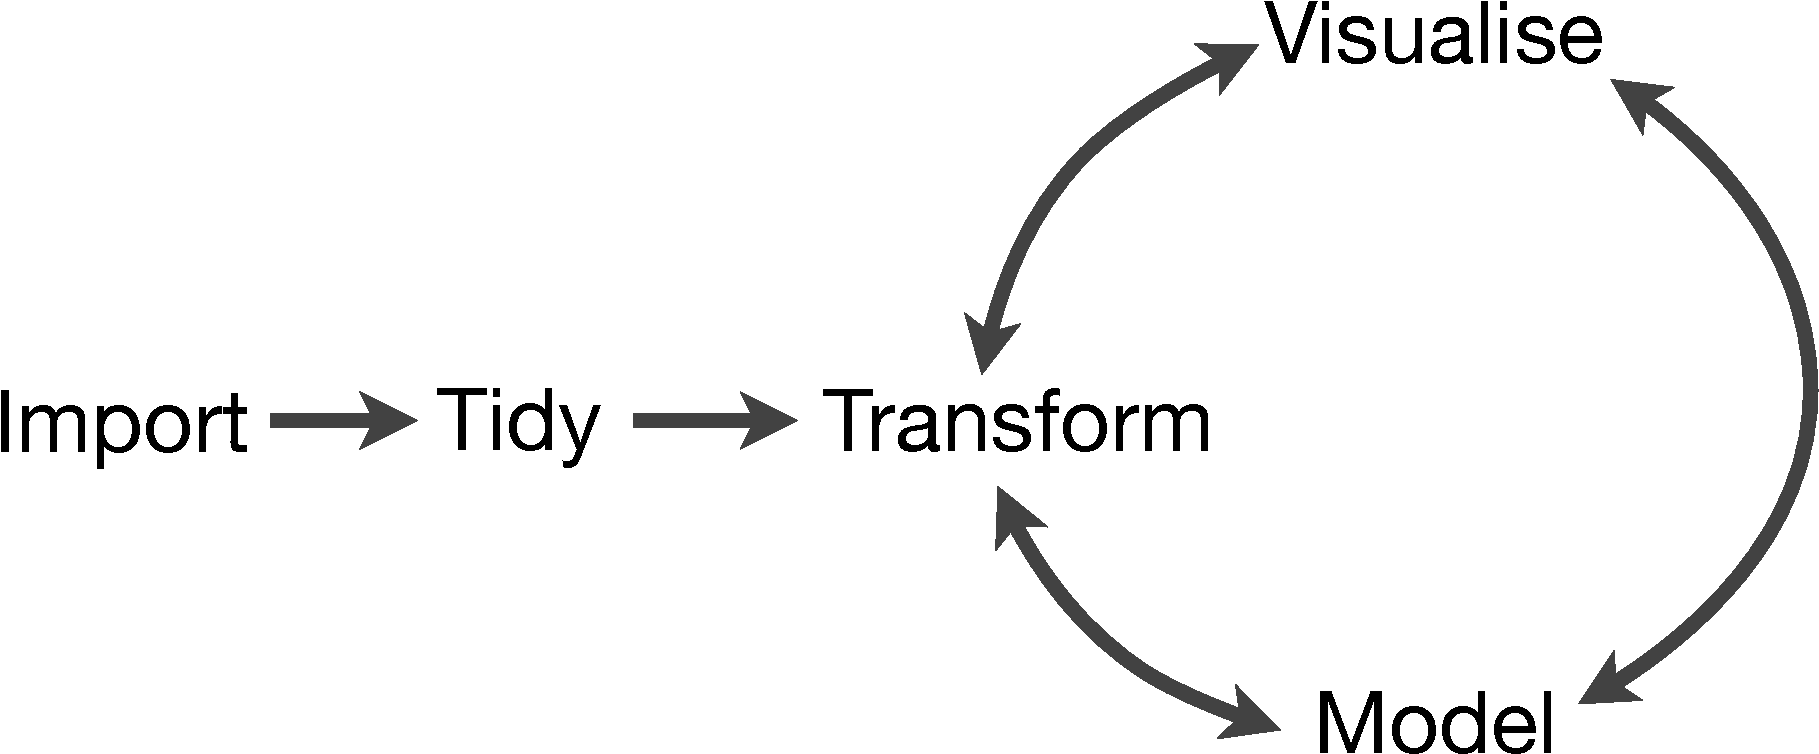
\includegraphics[height=1.2in]{cycle-crop}
  \caption{The data analysis cycle. First data is imported into the analysis environment and tidied into a form that's convenient to work with. Knowledge generation takes place with an iterative cycle of manipulation (e.g. creating new variables or summarising the data), visualisation and modelling.}
  \label{fig:cycle}
\end{figure}

The interplay between modeling and visualization, and the sometimes orthogonal role that visualization takes are described carefully in the introduction to \cite{cook:2007} (the pdf of the chapter is available free at \url{http://ggobi.org/book/intro.pdf}), \cite{Ch95}, and \cite{CH90}. Attention should also be drawn to data ``snooping" as practiced in the model selection process -- when we return and re-fit a new model technically this is using up degrees of freedom -- and the modeling world has tended to keep this swept under the carpet. Recent work \cite{berk:2013} and unpublished articles and software at \url{http://www-stat.wharton.upenn.edu/~buja/} provide some solutions.

Patil et al have missed the point on the all models perspective. Plotting a single scatterplot of living area and number of bedrooms hints at potential collinearity problems for model fitting, but the correlation does not look so strong, and looking at these two variables only negates the interplay between the multiple predictors. Given their arguments about the difficulty of perceiving correlation from a scatterplot, it's ironic that they'd use one for this purpose! The all models view tells us that the ``best'' models as measured by $R^2$ contain living area, and bedrooms, albeit having a practically difficult to explain negative coefficient for bedrooms. It says that bedrooms are important. Leek et al neglected to describe the next steps for the modeling, which are to partially regress bedrooms on living area and only consider the residuals from this fit as the predictor. Using the fitting the all models in the classroom would help new students better understand the complications arising from multiple predictors.

We disagree with the interpretation of \cite{Fisher}: we would argue that the assessment of statistical significance from a single plot is not important. This is what we have a statistical tests for. People tend to respond more closely to practical significance, and if the effect size in the relationship is large then people tend to see this. This is particularly important given the practically everything is statistically significance when you have a lot of data. We need visualization to both gauge practical significance and to spot the violations of model assumptions. In the third study of \cite{majumder:2013} subjects were asked to detect trend between two variables in the presence of contamination. A statistical test of the slope would report no significant trend but people do pick up on the trend. Humans are capable of ignoring contamination and focussing on common patterns.

% Villa-Vialaneix and co -------------------------------------------------------

\textbf{Villa-Vialaneix and Ruiz-Gazen (2015)} provide many additional examples to support the use of visualization in statistical practice, and like Allen et al point to the additional complexities afforded by data problems, especially networks and non-numeric variables. Their approach of averaging projections of a high-dimensional data set produced by multiple starts is innovative, and merits studying in more depth. We would suggest also looking at the projection coefficients from the different starts as a separate data set, much like the all models approach in our paper. By looking the distributions of these coefficients we might learn more about the high-dimensional function (kurtosis projection pursuit index), and whether the (local) maxima are primarily are in one location or two or more locations in the data space. Linking between displays of these coefficients and the projected data could provide more detail on what structure in the data was being detected by the function. We agree that it is still cumbersome to distribute interactive graphics, and this is an important area of research. The interactive graphics available in Villa-Vialaneix's sombrero shiny app are a step in the right direction.

% Hurley -----------------------------------------------------------------------

\textbf{Hurley (2015)} provides some excellent additional examples of algorithms that can be used to organize the object fed into the visualization, and points out the universal difficulty of installing interactive graphics software.

The dendrogram is a commonly used visualisation that displays the data in the model space. Hurley and collaborators have been doing innovative work to improve its fidelity. A thoughtful seriation (ordering of the nodes) considerably improves the visualisation by making it a closer match to the data space. This work is important not only because it improves upon a widely used visualisation (and one that has been around for many years), but also because the authors have endeavoured to make their work as easy to apply as possible. Accompanying research by an R package is an important way to get visualisation research into the hands of practitioners.

% Summary ----------------------------------------------------------------------

\textbf{In summary}, we very much appreciate the thoughtful and detailed discussions. This is an exciting time for visualization research, and the next frontier is better integration of modeling and graphics with easily accessible interactive graphics systems.

A common thread is the challenge of distributing interactive visualisations, and getting practices out of the hands of researchers and into the hands of practitioners. There is no doubt that software, and R packages in particular, are a fantastic tool for solving both problems. We are excited to see so many researchers embrace software development, and are excited at how tools for integrating R with the web make it easier than easier to distribute our work.

The integration of visualisation and modelling is a challenge that statisticians are uniquely positioned to face, and making in-roads in this area will continue to highlight statistics as one of the key tools of data science.

\bibliographystyle{abbrvnat}
\bibliography{../references}

\end{document}
